\documentclass[conference]{IEEEtran}
\IEEEoverridecommandlockouts
% The preceding line is only needed to identify funding in the first footnote. If that is unneeded, please comment it out.
\usepackage{cite}
\usepackage{amsmath,amssymb,amsfonts}
\usepackage{algorithmic}
\usepackage{graphicx}
\usepackage{textcomp}
\usepackage{xcolor}
\usepackage{tikz}
\usepackage{hyperref}

\def\BibTeX{{\rm B\kern-.05em{\sc i\kern-.025em b}\kern-.08em
    T\kern-.1667em\lower.7ex\hbox{E}\kern-.125emX}}
\begin{document}

\definecolor{myGreen}{RGB}{95,173,86}
\definecolor{myYellow}{RGB}{242,193,78}
\definecolor{myOrange}{RGB}{247,129,84}
\definecolor{myBlue}{RGB}{118,146,255}
\definecolor{myBrown}{RGB}{90,42,39}
\definecolor{myGrey}{RGB}{238, 228, 225}

\title{TensorStencil Report}

\author{\IEEEauthorblockN{Robert Buxton}
\IEEEauthorblockA{rb419@ic.ac.uk}

}

\maketitle

\begin{abstract}
Todo
\end{abstract}

\begin{IEEEkeywords}
Todo
\end{IEEEkeywords}


\section{Introduction}
Todo (Make better use of tensor cores/gpu matrix multipliers for stencil computation)
\section{Method}
I propose an alternative to the classical iterative loop method for stencil computation. 
Using the emergent properties of the transformation matrices use to represent stencil time step update we can calculate the state of input data after an arbitrary number of time steps. 

SOURCE THE PAPER BEFORE THE DIAGRAM \\

\newcommand{\gridCellWidth}{0.3}
\newcommand{\gridSize}{7}
\newcommand{\gridSpacing}{0.9}
\newcommand{\gridWidth}{\gridSize*\gridCellWidth}
\definecolor{myGreen}{RGB}{95,173,86}
\definecolor{myYellow}{RGB}{242,193,78}
\definecolor{myOrange}{RGB}{247,129,84}
\newcommand{\gridAxisHorizontalCellColour}{myGreen}
\newcommand{\gridAxisVerticalCellColour}{myOrange}
\newcommand{\gridAxisMiddleColour}{myYellow}
\newcommand{\gridTwoStart}{\gridWidth + \gridSpacing}
\newcommand{\gridThreeStart}{2*\gridWidth + 2*\gridSpacing}

\begin{tikzpicture}[every node/.style={minimum size=\gridCellWidth cm-\pgflinewidth, outer sep=0pt}]

%Grid 1

\draw[step=\gridCellWidth cm,color=black] (0,0) grid (\gridWidth,\gridWidth);

\node[fill={\gridAxisHorizontalCellColour}] at (1.5*\gridCellWidth,3.5*\gridCellWidth){};
\node[fill={\gridAxisHorizontalCellColour}] at (2.5*\gridCellWidth,3.5*\gridCellWidth){};
\node[fill={\gridAxisHorizontalCellColour}] at (4.5*\gridCellWidth,3.5*\gridCellWidth){};
\node[fill={\gridAxisHorizontalCellColour}] at (5.5*\gridCellWidth,3.5*\gridCellWidth){};


\node at (1.5*\gridCellWidth,3.5*\gridCellWidth) {\footnotesize x1};
\node at (2.5*\gridCellWidth,3.5*\gridCellWidth) {\footnotesize x2};
\node at (4.5*\gridCellWidth,3.5*\gridCellWidth) {\footnotesize x3};
\node at (5.5*\gridCellWidth,3.5*\gridCellWidth) {\footnotesize x4};


\node[fill={\gridAxisVerticalCellColour}] at (3.5*\gridCellWidth,1.5*\gridCellWidth){};
\node[fill={\gridAxisVerticalCellColour}] at (3.5*\gridCellWidth,2.5*\gridCellWidth){};
\node[fill={\gridAxisVerticalCellColour}] at (3.5*\gridCellWidth,4.5*\gridCellWidth){};
\node[fill={\gridAxisVerticalCellColour}] at (3.5*\gridCellWidth,5.5*\gridCellWidth){};

\node at (3.5*\gridCellWidth,1.5*\gridCellWidth) {\footnotesize y4};
\node at (3.5*\gridCellWidth,2.5*\gridCellWidth) {\footnotesize y3};
\node at (3.5*\gridCellWidth,4.5*\gridCellWidth) {\footnotesize y2};
\node at (3.5*\gridCellWidth,5.5*\gridCellWidth) {\footnotesize y1};


\node[fill={\gridAxisMiddleColour}] at (3.5*\gridCellWidth,3.5*\gridCellWidth){};

\node at (3.5*\gridCellWidth,3.5*\gridCellWidth) {\footnotesize m};

\node[fill={\gridAxisMiddleColour}] at (\gridTwoStart + 3.5*\gridCellWidth,3.5*\gridCellWidth){};
\node at (\gridTwoStart + 3.5*\gridCellWidth,3.5*\gridCellWidth) {\tiny{$\frac{\text{m}}{2}$} };

%Grid 2

\draw[step=\gridCellWidth cm,color=black] (\gridThreeStart,0) grid (\gridWidth + \gridThreeStart,\gridWidth);

\node[fill={\gridAxisVerticalCellColour}] at (\gridTwoStart + 3.5*\gridCellWidth,2.5*\gridCellWidth){};
\node[fill={\gridAxisVerticalCellColour}] at (\gridTwoStart + 3.5*\gridCellWidth,1.5*\gridCellWidth){};
\node[fill={\gridAxisVerticalCellColour}] at (\gridTwoStart + 3.5*\gridCellWidth,4.5*\gridCellWidth){};
\node[fill={\gridAxisVerticalCellColour}] at (\gridTwoStart + 3.5*\gridCellWidth,5.5*\gridCellWidth){};

\node at (\gridTwoStart + 3.5*\gridCellWidth,1.5*\gridCellWidth) {\footnotesize y4};
\node at (\gridTwoStart + 3.5*\gridCellWidth,2.5*\gridCellWidth) {\footnotesize y3};
\node at (\gridTwoStart + 3.5*\gridCellWidth,4.5*\gridCellWidth) {\footnotesize y2};
\node at (\gridTwoStart + 3.5*\gridCellWidth,5.5*\gridCellWidth) {\footnotesize y1};

%Grid 3

\draw[step=\gridCellWidth cm,color=black] (\gridTwoStart,0) grid (\gridWidth + \gridTwoStart,\gridWidth);

\node[fill={\gridAxisHorizontalCellColour}] at (\gridThreeStart + 1.5*\gridCellWidth,3.5*\gridCellWidth){};
\node[fill={\gridAxisHorizontalCellColour}] at (\gridThreeStart + 2.5*\gridCellWidth,3.5*\gridCellWidth){};
\node[fill={\gridAxisHorizontalCellColour}] at (\gridThreeStart + 4.5*\gridCellWidth,3.5*\gridCellWidth){};
\node[fill={\gridAxisHorizontalCellColour}] at (\gridThreeStart + 5.5*\gridCellWidth,3.5*\gridCellWidth){};

\node at (\gridThreeStart + 1.5*\gridCellWidth,3.5*\gridCellWidth) {\footnotesize x1};
\node at (\gridThreeStart + 2.5*\gridCellWidth,3.5*\gridCellWidth) {\footnotesize x2};
\node at (\gridThreeStart + 4.5*\gridCellWidth,3.5*\gridCellWidth) {\footnotesize x3};
\node at (\gridThreeStart + 5.5*\gridCellWidth,3.5*\gridCellWidth) {\footnotesize x4};


\node[fill={\gridAxisMiddleColour}] at (\gridThreeStart + 3.5*\gridCellWidth,3.5*\gridCellWidth){};
\node at (\gridThreeStart + 3.5*\gridCellWidth,3.5*\gridCellWidth) {\tiny{$\frac{\text{m}}{2}$} };


\node at (\gridWidth + \gridSpacing/2 ,3.5*\gridCellWidth){\large =};
\node at (\gridThreeStart - \gridSpacing/2 ,3.5*\gridCellWidth){\large +};

\end{tikzpicture} \\
\renewcommand{\gridCellWidth}{0.3}
\renewcommand{\gridSize}{7}
\renewcommand{\gridSpacing}{0.9}
\renewcommand{\gridWidth}{\gridSize*\gridCellWidth}
\renewcommand{\gridTwoStart}{\gridWidth + \gridSpacing}

\begin{tikzpicture}[every node/.style={minimum size=\gridCellWidth cm-\pgflinewidth, outer sep=0pt}]

%Grid 1

\draw[step=\gridCellWidth cm,color=black] (0,0) grid (\gridWidth,\gridWidth);

\node[fill={\gridAxisVerticalCellColour}] at (3.5*\gridCellWidth,1.5*\gridCellWidth){};
\node[fill={\gridAxisVerticalCellColour}] at (3.5*\gridCellWidth,2.5*\gridCellWidth){};
\node[fill={\gridAxisVerticalCellColour}] at (3.5*\gridCellWidth,4.5*\gridCellWidth){};
\node[fill={\gridAxisVerticalCellColour}] at (3.5*\gridCellWidth,5.5*\gridCellWidth){};

\node at (3.5*\gridCellWidth,1.5*\gridCellWidth) {\footnotesize y4};
\node at (3.5*\gridCellWidth,2.5*\gridCellWidth) {\footnotesize y3};
\node at (3.5*\gridCellWidth,4.5*\gridCellWidth) {\footnotesize y2};
\node at (3.5*\gridCellWidth,5.5*\gridCellWidth) {\footnotesize y1};

\node[fill={\gridAxisMiddleColour}] at (3.5*\gridCellWidth,3.5*\gridCellWidth){};

\node at (3.5*\gridCellWidth,3.5*\gridCellWidth) {\tiny{$\frac{\text{m}}{2}$}};

%Grid 2

\draw[step=\gridCellWidth cm,color=black] (\gridTwoStart,0) grid (\gridWidth + \gridTwoStart,\gridWidth);

\node[fill={\gridAxisVerticalCellColour}] at (\gridTwoStart + 0.5*\gridCellWidth,4.5*\gridCellWidth) {};
\node[fill={\gridAxisVerticalCellColour}] at (\gridTwoStart + 1.5*\gridCellWidth,3.5*\gridCellWidth) {};
\node[fill={\gridAxisVerticalCellColour}] at (\gridTwoStart + 2.5*\gridCellWidth,2.5*\gridCellWidth) {};
\node[fill={\gridAxisVerticalCellColour}] at (\gridTwoStart + 3.5*\gridCellWidth,1.5*\gridCellWidth) {};
\node[fill={\gridAxisVerticalCellColour}] at (\gridTwoStart + 4.5*\gridCellWidth,0.5*\gridCellWidth) {};

\node at (\gridTwoStart + 0.5*\gridCellWidth,4.5*\gridCellWidth) {\footnotesize y1};
\node at (\gridTwoStart + 1.5*\gridCellWidth,3.5*\gridCellWidth) {\footnotesize y1};
\node at (\gridTwoStart + 2.5*\gridCellWidth,2.5*\gridCellWidth) {\footnotesize y1};
\node at (\gridTwoStart + 3.5*\gridCellWidth,1.5*\gridCellWidth) {\footnotesize y1};
\node at (\gridTwoStart + 4.5*\gridCellWidth,0.5*\gridCellWidth) {\footnotesize y1};


\node[fill={\gridAxisVerticalCellColour}] at (\gridTwoStart + 0.5*\gridCellWidth,5.5*\gridCellWidth) {};
\node[fill={\gridAxisVerticalCellColour}] at (\gridTwoStart + 1.5*\gridCellWidth,4.5*\gridCellWidth) {};
\node[fill={\gridAxisVerticalCellColour}] at (\gridTwoStart + 2.5*\gridCellWidth,3.5*\gridCellWidth) {};
\node[fill={\gridAxisVerticalCellColour}] at (\gridTwoStart + 3.5*\gridCellWidth,2.5*\gridCellWidth) {};
\node[fill={\gridAxisVerticalCellColour}] at (\gridTwoStart + 4.5*\gridCellWidth,1.5*\gridCellWidth) {};
\node[fill={\gridAxisVerticalCellColour}] at (\gridTwoStart + 5.5*\gridCellWidth,0.5*\gridCellWidth) {};

\node at (\gridTwoStart + 0.5*\gridCellWidth,5.5*\gridCellWidth) {\footnotesize y2};
\node at (\gridTwoStart + 1.5*\gridCellWidth,4.5*\gridCellWidth) {\footnotesize y2};
\node at (\gridTwoStart + 2.5*\gridCellWidth,3.5*\gridCellWidth) {\footnotesize y2};
\node at (\gridTwoStart + 3.5*\gridCellWidth,2.5*\gridCellWidth) {\footnotesize y2};
\node at (\gridTwoStart + 4.5*\gridCellWidth,1.5*\gridCellWidth) {\footnotesize y2};
\node at (\gridTwoStart + 5.5*\gridCellWidth,0.5*\gridCellWidth) {\footnotesize y2};


\node[fill={\gridAxisMiddleColour}] at (\gridTwoStart + 0.5*\gridCellWidth,6.5*\gridCellWidth){};
\node[fill={\gridAxisMiddleColour}] at (\gridTwoStart + 1.5*\gridCellWidth,5.5*\gridCellWidth){};
\node[fill={\gridAxisMiddleColour}] at (\gridTwoStart + 2.5*\gridCellWidth,4.5*\gridCellWidth){};
\node[fill={\gridAxisMiddleColour}] at (\gridTwoStart + 3.5*\gridCellWidth,3.5*\gridCellWidth){};
\node[fill={\gridAxisMiddleColour}] at (\gridTwoStart + 4.5*\gridCellWidth,2.5*\gridCellWidth){};
\node[fill={\gridAxisMiddleColour}] at (\gridTwoStart + 5.5*\gridCellWidth,1.5*\gridCellWidth){};
\node[fill={\gridAxisMiddleColour}] at (\gridTwoStart + 6.5*\gridCellWidth,0.5*\gridCellWidth){};

\node at (\gridTwoStart + 0.5*\gridCellWidth,6.5*\gridCellWidth) {\tiny{$\frac{\text{m}}{2}$} };
\node at (\gridTwoStart + 1.5*\gridCellWidth,5.5*\gridCellWidth) {\tiny{$\frac{\text{m}}{2}$} };
\node at (\gridTwoStart + 2.5*\gridCellWidth,4.5*\gridCellWidth) {\tiny{$\frac{\text{m}}{2}$} };
\node at (\gridTwoStart + 3.5*\gridCellWidth,3.5*\gridCellWidth) {\tiny{$\frac{\text{m}}{2}$} };
\node at (\gridTwoStart + 4.5*\gridCellWidth,2.5*\gridCellWidth) {\tiny{$\frac{\text{m}}{2}$} };
\node at (\gridTwoStart + 5.5*\gridCellWidth,1.5*\gridCellWidth) {\tiny{$\frac{\text{m}}{2}$} };
\node at (\gridTwoStart + 6.5*\gridCellWidth,0.5*\gridCellWidth) {\tiny{$\frac{\text{m}}{2}$} };


\node[fill={\gridAxisVerticalCellColour}] at (\gridTwoStart + 1.5*\gridCellWidth,6.5*\gridCellWidth) {};
\node[fill={\gridAxisVerticalCellColour}] at (\gridTwoStart + 2.5*\gridCellWidth,5.5*\gridCellWidth) {};
\node[fill={\gridAxisVerticalCellColour}] at (\gridTwoStart + 3.5*\gridCellWidth,4.5*\gridCellWidth) {};
\node[fill={\gridAxisVerticalCellColour}] at (\gridTwoStart + 4.5*\gridCellWidth,3.5*\gridCellWidth) {};
\node[fill={\gridAxisVerticalCellColour}] at (\gridTwoStart + 5.5*\gridCellWidth,2.5*\gridCellWidth) {};
\node[fill={\gridAxisVerticalCellColour}] at (\gridTwoStart + 6.5*\gridCellWidth,1.5*\gridCellWidth) {};

\node at (\gridTwoStart + 1.5*\gridCellWidth,6.5*\gridCellWidth) {\footnotesize y3};
\node at (\gridTwoStart + 2.5*\gridCellWidth,5.5*\gridCellWidth) {\footnotesize y3};
\node at (\gridTwoStart + 3.5*\gridCellWidth,4.5*\gridCellWidth) {\footnotesize y3};
\node at (\gridTwoStart + 4.5*\gridCellWidth,3.5*\gridCellWidth) {\footnotesize y3};
\node at (\gridTwoStart + 5.5*\gridCellWidth,2.5*\gridCellWidth) {\footnotesize y3};
\node at (\gridTwoStart + 6.5*\gridCellWidth,1.5*\gridCellWidth) {\footnotesize y3};


\node[fill={\gridAxisVerticalCellColour}] at (\gridTwoStart + 2.5*\gridCellWidth,6.5*\gridCellWidth) {};
\node[fill={\gridAxisVerticalCellColour}] at (\gridTwoStart + 3.5*\gridCellWidth,5.5*\gridCellWidth) {};
\node[fill={\gridAxisVerticalCellColour}] at (\gridTwoStart + 4.5*\gridCellWidth,4.5*\gridCellWidth) {};
\node[fill={\gridAxisVerticalCellColour}] at (\gridTwoStart + 5.5*\gridCellWidth,3.5*\gridCellWidth) {};
\node[fill={\gridAxisVerticalCellColour}] at (\gridTwoStart + 6.5*\gridCellWidth,2.5*\gridCellWidth) {};

\node at (\gridTwoStart + 2.5*\gridCellWidth,6.5*\gridCellWidth) {\footnotesize y4};
\node at (\gridTwoStart + 3.5*\gridCellWidth,5.5*\gridCellWidth) {\footnotesize y4};
\node at (\gridTwoStart + 4.5*\gridCellWidth,4.5*\gridCellWidth) {\footnotesize y4};
\node at (\gridTwoStart + 5.5*\gridCellWidth,3.5*\gridCellWidth) {\footnotesize y4};
\node at (\gridTwoStart + 6.5*\gridCellWidth,2.5*\gridCellWidth) {\footnotesize y4};


% X and ->
\node at (\gridWidth + \gridSpacing/2 ,3.5*\gridCellWidth){\large $\rightarrow$};
\node at (\gridTwoStart + \gridWidth + \gridSpacing/2 ,3.5*\gridCellWidth){\large $\quad = Y $};


\end{tikzpicture} \\
\renewcommand{\gridCellWidth}{0.3}
\renewcommand{\gridSize}{7}
\renewcommand{\gridSpacing}{0.9}
\renewcommand{\gridWidth}{\gridSize*\gridCellWidth}
\renewcommand{\gridTwoStart}{\gridWidth + \gridSpacing}

\begin{tikzpicture}[every node/.style={minimum size=\gridCellWidth cm-\pgflinewidth, outer sep=0pt}]

%Grid 1

\draw[step=\gridCellWidth cm,color=black] (0,0) grid (\gridWidth,\gridWidth);

\node[fill={\gridAxisHorizontalCellColour}] at (1.5*\gridCellWidth,3.5*\gridCellWidth){};
\node[fill={\gridAxisHorizontalCellColour}] at (2.5*\gridCellWidth,3.5*\gridCellWidth){};
\node[fill={\gridAxisHorizontalCellColour}] at (4.5*\gridCellWidth,3.5*\gridCellWidth){};
\node[fill={\gridAxisHorizontalCellColour}] at (5.5*\gridCellWidth,3.5*\gridCellWidth){};

\node at (1.5*\gridCellWidth,3.5*\gridCellWidth) {\footnotesize x1};
\node at (2.5*\gridCellWidth,3.5*\gridCellWidth) {\footnotesize x2};
\node at (4.5*\gridCellWidth,3.5*\gridCellWidth) {\footnotesize x3};
\node at (5.5*\gridCellWidth,3.5*\gridCellWidth) {\footnotesize x4};

\node[fill={\gridAxisMiddleColour}] at (3.5*\gridCellWidth,3.5*\gridCellWidth){};

\node at (3.5*\gridCellWidth,3.5*\gridCellWidth) {\tiny{$\frac{\text{m}}{2}$}};

%Grid 2

\draw[step=\gridCellWidth cm,color=black] (\gridTwoStart,0) grid (\gridWidth + \gridTwoStart,\gridWidth);

\node[fill={\gridAxisHorizontalCellColour}] at (\gridTwoStart + 0.5*\gridCellWidth,4.5*\gridCellWidth) {};
\node[fill={\gridAxisHorizontalCellColour}] at (\gridTwoStart + 1.5*\gridCellWidth,3.5*\gridCellWidth) {};
\node[fill={\gridAxisHorizontalCellColour}] at (\gridTwoStart + 2.5*\gridCellWidth,2.5*\gridCellWidth) {};
\node[fill={\gridAxisHorizontalCellColour}] at (\gridTwoStart + 3.5*\gridCellWidth,1.5*\gridCellWidth) {};
\node[fill={\gridAxisHorizontalCellColour}] at (\gridTwoStart + 4.5*\gridCellWidth,0.5*\gridCellWidth) {};

\node at (\gridTwoStart + 0.5*\gridCellWidth,4.5*\gridCellWidth) {\footnotesize x1};
\node at (\gridTwoStart + 1.5*\gridCellWidth,3.5*\gridCellWidth) {\footnotesize x1};
\node at (\gridTwoStart + 2.5*\gridCellWidth,2.5*\gridCellWidth) {\footnotesize x1};
\node at (\gridTwoStart + 3.5*\gridCellWidth,1.5*\gridCellWidth) {\footnotesize x1};
\node at (\gridTwoStart + 4.5*\gridCellWidth,0.5*\gridCellWidth) {\footnotesize x1};


\node[fill={\gridAxisHorizontalCellColour}] at (\gridTwoStart + 0.5*\gridCellWidth,5.5*\gridCellWidth) {};
\node[fill={\gridAxisHorizontalCellColour}] at (\gridTwoStart + 1.5*\gridCellWidth,4.5*\gridCellWidth) {};
\node[fill={\gridAxisHorizontalCellColour}] at (\gridTwoStart + 2.5*\gridCellWidth,3.5*\gridCellWidth) {};
\node[fill={\gridAxisHorizontalCellColour}] at (\gridTwoStart + 3.5*\gridCellWidth,2.5*\gridCellWidth) {};
\node[fill={\gridAxisHorizontalCellColour}] at (\gridTwoStart + 4.5*\gridCellWidth,1.5*\gridCellWidth) {};
\node[fill={\gridAxisHorizontalCellColour}] at (\gridTwoStart + 5.5*\gridCellWidth,0.5*\gridCellWidth) {};

\node at (\gridTwoStart + 0.5*\gridCellWidth,5.5*\gridCellWidth) {\footnotesize x2};
\node at (\gridTwoStart + 1.5*\gridCellWidth,4.5*\gridCellWidth) {\footnotesize x2};
\node at (\gridTwoStart + 2.5*\gridCellWidth,3.5*\gridCellWidth) {\footnotesize x2};
\node at (\gridTwoStart + 3.5*\gridCellWidth,2.5*\gridCellWidth) {\footnotesize x2};
\node at (\gridTwoStart + 4.5*\gridCellWidth,1.5*\gridCellWidth) {\footnotesize x2};
\node at (\gridTwoStart + 5.5*\gridCellWidth,0.5*\gridCellWidth) {\footnotesize x2};


\node[fill={\gridAxisMiddleColour}] at (\gridTwoStart + 0.5*\gridCellWidth,6.5*\gridCellWidth){};
\node[fill={\gridAxisMiddleColour}] at (\gridTwoStart + 1.5*\gridCellWidth,5.5*\gridCellWidth){};
\node[fill={\gridAxisMiddleColour}] at (\gridTwoStart + 2.5*\gridCellWidth,4.5*\gridCellWidth){};
\node[fill={\gridAxisMiddleColour}] at (\gridTwoStart + 3.5*\gridCellWidth,3.5*\gridCellWidth){};
\node[fill={\gridAxisMiddleColour}] at (\gridTwoStart + 4.5*\gridCellWidth,2.5*\gridCellWidth){};
\node[fill={\gridAxisMiddleColour}] at (\gridTwoStart + 5.5*\gridCellWidth,1.5*\gridCellWidth){};
\node[fill={\gridAxisMiddleColour}] at (\gridTwoStart + 6.5*\gridCellWidth,0.5*\gridCellWidth){};

\node at (\gridTwoStart + 0.5*\gridCellWidth,6.5*\gridCellWidth) {\tiny{$\frac{\text{m}}{2}$} };
\node at (\gridTwoStart + 1.5*\gridCellWidth,5.5*\gridCellWidth) {\tiny{$\frac{\text{m}}{2}$} };
\node at (\gridTwoStart + 2.5*\gridCellWidth,4.5*\gridCellWidth) {\tiny{$\frac{\text{m}}{2}$} };
\node at (\gridTwoStart + 3.5*\gridCellWidth,3.5*\gridCellWidth) {\tiny{$\frac{\text{m}}{2}$} };
\node at (\gridTwoStart + 4.5*\gridCellWidth,2.5*\gridCellWidth) {\tiny{$\frac{\text{m}}{2}$} };
\node at (\gridTwoStart + 5.5*\gridCellWidth,1.5*\gridCellWidth) {\tiny{$\frac{\text{m}}{2}$} };
\node at (\gridTwoStart + 6.5*\gridCellWidth,0.5*\gridCellWidth) {\tiny{$\frac{\text{m}}{2}$} };


\node[fill={\gridAxisHorizontalCellColour}] at (\gridTwoStart + 1.5*\gridCellWidth,6.5*\gridCellWidth) {};
\node[fill={\gridAxisHorizontalCellColour}] at (\gridTwoStart + 2.5*\gridCellWidth,5.5*\gridCellWidth) {};
\node[fill={\gridAxisHorizontalCellColour}] at (\gridTwoStart + 3.5*\gridCellWidth,4.5*\gridCellWidth) {};
\node[fill={\gridAxisHorizontalCellColour}] at (\gridTwoStart + 4.5*\gridCellWidth,3.5*\gridCellWidth) {};
\node[fill={\gridAxisHorizontalCellColour}] at (\gridTwoStart + 5.5*\gridCellWidth,2.5*\gridCellWidth) {};
\node[fill={\gridAxisHorizontalCellColour}] at (\gridTwoStart + 6.5*\gridCellWidth,1.5*\gridCellWidth) {};

\node at (\gridTwoStart + 1.5*\gridCellWidth,6.5*\gridCellWidth) {\footnotesize x3};
\node at (\gridTwoStart + 2.5*\gridCellWidth,5.5*\gridCellWidth) {\footnotesize x3};
\node at (\gridTwoStart + 3.5*\gridCellWidth,4.5*\gridCellWidth) {\footnotesize x3};
\node at (\gridTwoStart + 4.5*\gridCellWidth,3.5*\gridCellWidth) {\footnotesize x3};
\node at (\gridTwoStart + 5.5*\gridCellWidth,2.5*\gridCellWidth) {\footnotesize x3};
\node at (\gridTwoStart + 6.5*\gridCellWidth,1.5*\gridCellWidth) {\footnotesize x3};


\node[fill={\gridAxisHorizontalCellColour}] at (\gridTwoStart + 2.5*\gridCellWidth,6.5*\gridCellWidth) {};
\node[fill={\gridAxisHorizontalCellColour}] at (\gridTwoStart + 3.5*\gridCellWidth,5.5*\gridCellWidth) {};
\node[fill={\gridAxisHorizontalCellColour}] at (\gridTwoStart + 4.5*\gridCellWidth,4.5*\gridCellWidth) {};
\node[fill={\gridAxisHorizontalCellColour}] at (\gridTwoStart + 5.5*\gridCellWidth,3.5*\gridCellWidth) {};
\node[fill={\gridAxisHorizontalCellColour}] at (\gridTwoStart + 6.5*\gridCellWidth,2.5*\gridCellWidth) {};

\node at (\gridTwoStart + 2.5*\gridCellWidth,6.5*\gridCellWidth) {\footnotesize x4};
\node at (\gridTwoStart + 3.5*\gridCellWidth,5.5*\gridCellWidth) {\footnotesize x4};
\node at (\gridTwoStart + 4.5*\gridCellWidth,4.5*\gridCellWidth) {\footnotesize x4};
\node at (\gridTwoStart + 5.5*\gridCellWidth,3.5*\gridCellWidth) {\footnotesize x4};
\node at (\gridTwoStart + 6.5*\gridCellWidth,2.5*\gridCellWidth) {\footnotesize x4};


% Y and ->
\node at (\gridWidth + \gridSpacing/2 ,3.5*\gridCellWidth){\large $\rightarrow$};
\node at (\gridTwoStart + \gridWidth + \gridSpacing/2 ,3.5*\gridCellWidth){\large $\quad = X $};

\end{tikzpicture} \\
\renewcommand{\gridCellWidth}{0.3}
\renewcommand{\gridSize}{7}
\renewcommand{\gridSpacing}{1.5}
\renewcommand{\gridWidth}{\gridSize*\gridCellWidth}
\renewcommand{\gridAxisHorizontalCellColour}{myGreen}
\renewcommand{\gridAxisVerticalCellColour}{myOrange}
\renewcommand{\gridAxisMiddleColour}{myYellow}
\renewcommand{\gridTwoStart}{\gridSpacing}
\renewcommand{\gridThreeStart}{\gridTwoStart + \gridWidth + \gridSpacing}



\begin{tikzpicture}[every node/.style={minimum size=\gridCellWidth cm-\pgflinewidth, outer sep=0pt}]

%Grid 1

\node at (\gridSpacing/2,3.5*\gridCellWidth) {\large $A_{t+1} =$};

%Grid 2

\draw[step=\gridCellWidth cm,color=black] (\gridTwoStart,0) grid (\gridWidth + \gridTwoStart,\gridWidth);

\node[fill={\gridAxisVerticalCellColour}] at (\gridTwoStart + 0.5*\gridCellWidth,4.5*\gridCellWidth) {};
\node[fill={\gridAxisVerticalCellColour}] at (\gridTwoStart + 1.5*\gridCellWidth,3.5*\gridCellWidth) {};
\node[fill={\gridAxisVerticalCellColour}] at (\gridTwoStart + 2.5*\gridCellWidth,2.5*\gridCellWidth) {};
\node[fill={\gridAxisVerticalCellColour}] at (\gridTwoStart + 3.5*\gridCellWidth,1.5*\gridCellWidth) {};
\node[fill={\gridAxisVerticalCellColour}] at (\gridTwoStart + 4.5*\gridCellWidth,0.5*\gridCellWidth) {};

\node at (\gridTwoStart + 0.5*\gridCellWidth,4.5*\gridCellWidth) {\footnotesize y1};
\node at (\gridTwoStart + 1.5*\gridCellWidth,3.5*\gridCellWidth) {\footnotesize y1};
\node at (\gridTwoStart + 2.5*\gridCellWidth,2.5*\gridCellWidth) {\footnotesize y1};
\node at (\gridTwoStart + 3.5*\gridCellWidth,1.5*\gridCellWidth) {\footnotesize y1};
\node at (\gridTwoStart + 4.5*\gridCellWidth,0.5*\gridCellWidth) {\footnotesize y1};


\node[fill={\gridAxisVerticalCellColour}] at (\gridTwoStart + 0.5*\gridCellWidth,5.5*\gridCellWidth) {};
\node[fill={\gridAxisVerticalCellColour}] at (\gridTwoStart + 1.5*\gridCellWidth,4.5*\gridCellWidth) {};
\node[fill={\gridAxisVerticalCellColour}] at (\gridTwoStart + 2.5*\gridCellWidth,3.5*\gridCellWidth) {};
\node[fill={\gridAxisVerticalCellColour}] at (\gridTwoStart + 3.5*\gridCellWidth,2.5*\gridCellWidth) {};
\node[fill={\gridAxisVerticalCellColour}] at (\gridTwoStart + 4.5*\gridCellWidth,1.5*\gridCellWidth) {};
\node[fill={\gridAxisVerticalCellColour}] at (\gridTwoStart + 5.5*\gridCellWidth,0.5*\gridCellWidth) {};

\node at (\gridTwoStart + 0.5*\gridCellWidth,5.5*\gridCellWidth) {\footnotesize y2};
\node at (\gridTwoStart + 1.5*\gridCellWidth,4.5*\gridCellWidth) {\footnotesize y2};
\node at (\gridTwoStart + 2.5*\gridCellWidth,3.5*\gridCellWidth) {\footnotesize y2};
\node at (\gridTwoStart + 3.5*\gridCellWidth,2.5*\gridCellWidth) {\footnotesize y2};
\node at (\gridTwoStart + 4.5*\gridCellWidth,1.5*\gridCellWidth) {\footnotesize y2};
\node at (\gridTwoStart + 5.5*\gridCellWidth,0.5*\gridCellWidth) {\footnotesize y2};


\node[fill={\gridAxisMiddleColour}] at (\gridTwoStart + 0.5*\gridCellWidth,6.5*\gridCellWidth){};
\node[fill={\gridAxisMiddleColour}] at (\gridTwoStart + 1.5*\gridCellWidth,5.5*\gridCellWidth){};
\node[fill={\gridAxisMiddleColour}] at (\gridTwoStart + 2.5*\gridCellWidth,4.5*\gridCellWidth){};
\node[fill={\gridAxisMiddleColour}] at (\gridTwoStart + 3.5*\gridCellWidth,3.5*\gridCellWidth){};
\node[fill={\gridAxisMiddleColour}] at (\gridTwoStart + 4.5*\gridCellWidth,2.5*\gridCellWidth){};
\node[fill={\gridAxisMiddleColour}] at (\gridTwoStart + 5.5*\gridCellWidth,1.5*\gridCellWidth){};
\node[fill={\gridAxisMiddleColour}] at (\gridTwoStart + 6.5*\gridCellWidth,0.5*\gridCellWidth){};

\node at (\gridTwoStart + 0.5*\gridCellWidth,6.5*\gridCellWidth) {\tiny{$\frac{\text{m}}{2}$} };
\node at (\gridTwoStart + 1.5*\gridCellWidth,5.5*\gridCellWidth) {\tiny{$\frac{\text{m}}{2}$} };
\node at (\gridTwoStart + 2.5*\gridCellWidth,4.5*\gridCellWidth) {\tiny{$\frac{\text{m}}{2}$} };
\node at (\gridTwoStart + 3.5*\gridCellWidth,3.5*\gridCellWidth) {\tiny{$\frac{\text{m}}{2}$} };
\node at (\gridTwoStart + 4.5*\gridCellWidth,2.5*\gridCellWidth) {\tiny{$\frac{\text{m}}{2}$} };
\node at (\gridTwoStart + 5.5*\gridCellWidth,1.5*\gridCellWidth) {\tiny{$\frac{\text{m}}{2}$} };
\node at (\gridTwoStart + 6.5*\gridCellWidth,0.5*\gridCellWidth) {\tiny{$\frac{\text{m}}{2}$} };


\node[fill={\gridAxisVerticalCellColour}] at (\gridTwoStart + 1.5*\gridCellWidth,6.5*\gridCellWidth) {};
\node[fill={\gridAxisVerticalCellColour}] at (\gridTwoStart + 2.5*\gridCellWidth,5.5*\gridCellWidth) {};
\node[fill={\gridAxisVerticalCellColour}] at (\gridTwoStart + 3.5*\gridCellWidth,4.5*\gridCellWidth) {};
\node[fill={\gridAxisVerticalCellColour}] at (\gridTwoStart + 4.5*\gridCellWidth,3.5*\gridCellWidth) {};
\node[fill={\gridAxisVerticalCellColour}] at (\gridTwoStart + 5.5*\gridCellWidth,2.5*\gridCellWidth) {};
\node[fill={\gridAxisVerticalCellColour}] at (\gridTwoStart + 6.5*\gridCellWidth,1.5*\gridCellWidth) {};

\node at (\gridTwoStart + 1.5*\gridCellWidth,6.5*\gridCellWidth) {\footnotesize y3};
\node at (\gridTwoStart + 2.5*\gridCellWidth,5.5*\gridCellWidth) {\footnotesize y3};
\node at (\gridTwoStart + 3.5*\gridCellWidth,4.5*\gridCellWidth) {\footnotesize y3};
\node at (\gridTwoStart + 4.5*\gridCellWidth,3.5*\gridCellWidth) {\footnotesize y3};
\node at (\gridTwoStart + 5.5*\gridCellWidth,2.5*\gridCellWidth) {\footnotesize y3};
\node at (\gridTwoStart + 6.5*\gridCellWidth,1.5*\gridCellWidth) {\footnotesize y3};


\node[fill={\gridAxisVerticalCellColour}] at (\gridTwoStart + 2.5*\gridCellWidth,6.5*\gridCellWidth) {};
\node[fill={\gridAxisVerticalCellColour}] at (\gridTwoStart + 3.5*\gridCellWidth,5.5*\gridCellWidth) {};
\node[fill={\gridAxisVerticalCellColour}] at (\gridTwoStart + 4.5*\gridCellWidth,4.5*\gridCellWidth) {};
\node[fill={\gridAxisVerticalCellColour}] at (\gridTwoStart + 5.5*\gridCellWidth,3.5*\gridCellWidth) {};
\node[fill={\gridAxisVerticalCellColour}] at (\gridTwoStart + 6.5*\gridCellWidth,2.5*\gridCellWidth) {};

\node at (\gridTwoStart + 2.5*\gridCellWidth,6.5*\gridCellWidth) {\footnotesize y4};
\node at (\gridTwoStart + 3.5*\gridCellWidth,5.5*\gridCellWidth) {\footnotesize y4};
\node at (\gridTwoStart + 4.5*\gridCellWidth,4.5*\gridCellWidth) {\footnotesize y4};
\node at (\gridTwoStart + 5.5*\gridCellWidth,3.5*\gridCellWidth) {\footnotesize y4};
\node at (\gridTwoStart + 6.5*\gridCellWidth,2.5*\gridCellWidth) {\footnotesize y4};

%Grid 3

\draw[step=\gridCellWidth cm,color=black] (\gridThreeStart,0) grid (\gridWidth + \gridThreeStart,\gridWidth);

\node[fill={\gridAxisHorizontalCellColour}] at (\gridThreeStart + 0.5*\gridCellWidth,4.5*\gridCellWidth) {};
\node[fill={\gridAxisHorizontalCellColour}] at (\gridThreeStart + 1.5*\gridCellWidth,3.5*\gridCellWidth) {};
\node[fill={\gridAxisHorizontalCellColour}] at (\gridThreeStart + 2.5*\gridCellWidth,2.5*\gridCellWidth) {};
\node[fill={\gridAxisHorizontalCellColour}] at (\gridThreeStart + 3.5*\gridCellWidth,1.5*\gridCellWidth) {};
\node[fill={\gridAxisHorizontalCellColour}] at (\gridThreeStart + 4.5*\gridCellWidth,0.5*\gridCellWidth) {};

\node at (\gridThreeStart + 0.5*\gridCellWidth,4.5*\gridCellWidth) {\footnotesize x1};
\node at (\gridThreeStart + 1.5*\gridCellWidth,3.5*\gridCellWidth) {\footnotesize x1};
\node at (\gridThreeStart + 2.5*\gridCellWidth,2.5*\gridCellWidth) {\footnotesize x1};
\node at (\gridThreeStart + 3.5*\gridCellWidth,1.5*\gridCellWidth) {\footnotesize x1};
\node at (\gridThreeStart + 4.5*\gridCellWidth,0.5*\gridCellWidth) {\footnotesize x1};

\node[fill={\gridAxisHorizontalCellColour}] at (\gridThreeStart + 0.5*\gridCellWidth,5.5*\gridCellWidth) {};
\node[fill={\gridAxisHorizontalCellColour}] at (\gridThreeStart + 1.5*\gridCellWidth,4.5*\gridCellWidth) {};
\node[fill={\gridAxisHorizontalCellColour}] at (\gridThreeStart + 2.5*\gridCellWidth,3.5*\gridCellWidth) {};
\node[fill={\gridAxisHorizontalCellColour}] at (\gridThreeStart + 3.5*\gridCellWidth,2.5*\gridCellWidth) {};
\node[fill={\gridAxisHorizontalCellColour}] at (\gridThreeStart + 4.5*\gridCellWidth,1.5*\gridCellWidth) {};
\node[fill={\gridAxisHorizontalCellColour}] at (\gridThreeStart + 5.5*\gridCellWidth,0.5*\gridCellWidth) {};

\node at (\gridThreeStart + 0.5*\gridCellWidth,5.5*\gridCellWidth) {\footnotesize x2};
\node at (\gridThreeStart + 1.5*\gridCellWidth,4.5*\gridCellWidth) {\footnotesize x2};
\node at (\gridThreeStart + 2.5*\gridCellWidth,3.5*\gridCellWidth) {\footnotesize x2};
\node at (\gridThreeStart + 3.5*\gridCellWidth,2.5*\gridCellWidth) {\footnotesize x2};
\node at (\gridThreeStart + 4.5*\gridCellWidth,1.5*\gridCellWidth) {\footnotesize x2};
\node at (\gridThreeStart + 5.5*\gridCellWidth,0.5*\gridCellWidth) {\footnotesize x2};


\node[fill={\gridAxisMiddleColour}] at (\gridThreeStart + 0.5*\gridCellWidth,6.5*\gridCellWidth){};
\node[fill={\gridAxisMiddleColour}] at (\gridThreeStart + 1.5*\gridCellWidth,5.5*\gridCellWidth){};
\node[fill={\gridAxisMiddleColour}] at (\gridThreeStart + 2.5*\gridCellWidth,4.5*\gridCellWidth){};
\node[fill={\gridAxisMiddleColour}] at (\gridThreeStart + 3.5*\gridCellWidth,3.5*\gridCellWidth){};
\node[fill={\gridAxisMiddleColour}] at (\gridThreeStart + 4.5*\gridCellWidth,2.5*\gridCellWidth){};
\node[fill={\gridAxisMiddleColour}] at (\gridThreeStart + 5.5*\gridCellWidth,1.5*\gridCellWidth){};
\node[fill={\gridAxisMiddleColour}] at (\gridThreeStart + 6.5*\gridCellWidth,0.5*\gridCellWidth){};

\node at (\gridThreeStart + 0.5*\gridCellWidth,6.5*\gridCellWidth) {\tiny{$\frac{\text{m}}{2}$} };
\node at (\gridThreeStart + 1.5*\gridCellWidth,5.5*\gridCellWidth) {\tiny{$\frac{\text{m}}{2}$} };
\node at (\gridThreeStart + 2.5*\gridCellWidth,4.5*\gridCellWidth) {\tiny{$\frac{\text{m}}{2}$} };
\node at (\gridThreeStart + 3.5*\gridCellWidth,3.5*\gridCellWidth) {\tiny{$\frac{\text{m}}{2}$} };
\node at (\gridThreeStart + 4.5*\gridCellWidth,2.5*\gridCellWidth) {\tiny{$\frac{\text{m}}{2}$} };
\node at (\gridThreeStart + 5.5*\gridCellWidth,1.5*\gridCellWidth) {\tiny{$\frac{\text{m}}{2}$} };
\node at (\gridThreeStart + 6.5*\gridCellWidth,0.5*\gridCellWidth) {\tiny{$\frac{\text{m}}{2}$} };


\node[fill={\gridAxisHorizontalCellColour}] at (\gridThreeStart + 1.5*\gridCellWidth,6.5*\gridCellWidth) {};
\node[fill={\gridAxisHorizontalCellColour}] at (\gridThreeStart + 2.5*\gridCellWidth,5.5*\gridCellWidth) {};
\node[fill={\gridAxisHorizontalCellColour}] at (\gridThreeStart + 3.5*\gridCellWidth,4.5*\gridCellWidth) {};
\node[fill={\gridAxisHorizontalCellColour}] at (\gridThreeStart + 4.5*\gridCellWidth,3.5*\gridCellWidth) {};
\node[fill={\gridAxisHorizontalCellColour}] at (\gridThreeStart + 5.5*\gridCellWidth,2.5*\gridCellWidth) {};
\node[fill={\gridAxisHorizontalCellColour}] at (\gridThreeStart + 6.5*\gridCellWidth,1.5*\gridCellWidth) {};

\node at (\gridThreeStart + 1.5*\gridCellWidth,6.5*\gridCellWidth) {\footnotesize x3};
\node at (\gridThreeStart + 2.5*\gridCellWidth,5.5*\gridCellWidth) {\footnotesize x3};
\node at (\gridThreeStart + 3.5*\gridCellWidth,4.5*\gridCellWidth) {\footnotesize x3};
\node at (\gridThreeStart + 4.5*\gridCellWidth,3.5*\gridCellWidth) {\footnotesize x3};
\node at (\gridThreeStart + 5.5*\gridCellWidth,2.5*\gridCellWidth) {\footnotesize x3};
\node at (\gridThreeStart + 6.5*\gridCellWidth,1.5*\gridCellWidth) {\footnotesize x3};


\node[fill={\gridAxisHorizontalCellColour}] at (\gridThreeStart + 2.5*\gridCellWidth,6.5*\gridCellWidth) {};
\node[fill={\gridAxisHorizontalCellColour}] at (\gridThreeStart + 3.5*\gridCellWidth,5.5*\gridCellWidth) {};
\node[fill={\gridAxisHorizontalCellColour}] at (\gridThreeStart + 4.5*\gridCellWidth,4.5*\gridCellWidth) {};
\node[fill={\gridAxisHorizontalCellColour}] at (\gridThreeStart + 5.5*\gridCellWidth,3.5*\gridCellWidth) {};
\node[fill={\gridAxisHorizontalCellColour}] at (\gridThreeStart + 6.5*\gridCellWidth,2.5*\gridCellWidth) {};

\node at (\gridThreeStart + 2.5*\gridCellWidth,6.5*\gridCellWidth) {\footnotesize x4};
\node at (\gridThreeStart + 3.5*\gridCellWidth,5.5*\gridCellWidth) {\footnotesize x4};
\node at (\gridThreeStart + 4.5*\gridCellWidth,4.5*\gridCellWidth) {\footnotesize x4};
\node at (\gridThreeStart + 5.5*\gridCellWidth,3.5*\gridCellWidth) {\footnotesize x4};
\node at (\gridThreeStart + 6.5*\gridCellWidth,2.5*\gridCellWidth) {\footnotesize x4};

%in between
\node at (\gridTwoStart + \gridWidth + \gridSpacing/2 ,3.5*\gridCellWidth){$\cdot A_t + A_t \cdot$};

% transpose
\node at (\gridThreeStart + \gridWidth + 0.2,\gridWidth){$T$};
\end{tikzpicture} \\

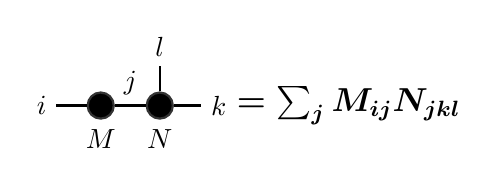
\begin{tikzpicture}
	\node[circle,draw=black!80,thick,fill=black,label=below:$M$] (M) at (0.75,0) {};
	\node[circle,draw=black!80,thick,fill=black,label=below:$N$] (N) at (1.5,0) {};
	\node (i) at (0,0) {$i$};
	\node (l) at (1.5,0.75) {$l$};
	\node (k) at (2.25,0) {$k$};
	\draw[thick, draw=black,label=above:] (M) -- node [above] {$j$} (N) {};
	\draw[thick, draw=black] (i) -- (M) {};
	\draw[thick, draw=black] (N) -- (k) {};
	\draw[thick, draw=black] (N) -- (l) {};
	\node at (3.9,0) {\large {\boldmath$= \sum_j M_{ij}N_{jkl}$}};
\end{tikzpicture}
 \\
\newcommand{\graphLineSpacing}{0.5}
\newcommand{\graphTensorSpacing}{1}
\newcommand{\graphTensorTwoStart}{1.5*\graphTensorSpacing}
\newcommand{\graphTensorThreeStart}{\graphTensorTwoStart+ 2*\graphTensorSpacing}
\newcommand{\graphTensorFourStart}{\graphTensorThreeStart+ 2*\graphTensorSpacing}

\begin{tikzpicture}
	\node[circle,draw=black!80,thick,fill=black,label=left:$A_{t+1}$] (ATT) at (0,0) {};
	\node[circle,draw=black!80,thick,fill=black,label=left:${=}A_{t}$] (AT) at (\graphTensorTwoStart,0) {};
	\node[circle,draw=black!80,thick,fill=myGreen,label=above right:$X$] (X) at (\graphTensorTwoStart + \graphLineSpacing,\graphLineSpacing) {};
	\node[circle,draw=black!80,thick,fill=black,label=left:$+A_{t}$] (A) at (\graphTensorThreeStart,0) {};
	\node[circle,draw=black!80,thick,fill=myOrange,label=above right:$Y$] (Y) at (\graphTensorThreeStart + \graphLineSpacing,-\graphLineSpacing) {};

	\draw[thick, draw=black] (ATT) -- (0,\graphLineSpacing) -- (\graphLineSpacing,\graphLineSpacing) {};
	\draw[thick, draw=black] (ATT) -- (0,-\graphLineSpacing) -- (\graphLineSpacing,-\graphLineSpacing) {};

	\draw[thick, draw=black] (AT) -- (\graphTensorTwoStart,\graphLineSpacing) -- (X) -- (\graphTensorTwoStart + 2*\graphLineSpacing,\graphLineSpacing) {};
	\draw[thick, draw=black] (AT) -- (\graphTensorTwoStart,-\graphLineSpacing) -- (\graphTensorTwoStart + \graphLineSpacing, -\graphLineSpacing) {};

	\draw[thick, draw=black] (A) -- (\graphTensorThreeStart,\graphLineSpacing) -- (\graphTensorThreeStart + \graphLineSpacing,\graphLineSpacing) {};
	\draw[thick, draw=black] (A) -- (\graphTensorThreeStart,-\graphLineSpacing) -- (Y) -- (\graphTensorThreeStart + 2*\graphLineSpacing,-\graphLineSpacing) {};
\end{tikzpicture}
\renewcommand{\graphTensorSpacing}{1.1}
\renewcommand{\graphTensorTwoStart}{1.5*\graphTensorSpacing}
\renewcommand{\graphTensorThreeStart}{\graphTensorTwoStart+ 2*\graphTensorSpacing}
\renewcommand{\graphTensorFourStart}{\graphTensorThreeStart+ 2*\graphTensorSpacing}

\begin{tikzpicture}
	\node[circle,draw=black!80,thick,fill=black,label=left:$A_{t+2}$] (ATWO) at (0,0) {};
	\node[circle,draw=black!80,thick,fill=black,label=left:${=} A_{t}$] (A) at (\graphTensorTwoStart,0) {};
	\node[circle,draw=black!80,thick,fill=myGreen,label=above right:$X$] (X) at (\graphTensorTwoStart + \graphLineSpacing,\graphLineSpacing) {};
	\node[circle,draw=black!80,thick,fill=myGreen,label=above right:$X$] (X2) at (\graphTensorTwoStart + 2*\graphLineSpacing,\graphLineSpacing) {};
	\node[circle,draw=black!80,thick,fill=black,label=left:$+2A_{t}$] (AT) at (\graphTensorThreeStart,0) {};
	\node[circle,draw=black!80,thick,fill=myGreen,label=above right:$X$] (X3) at (\graphTensorThreeStart + \graphLineSpacing,\graphLineSpacing) {};
	\node[circle,draw=black!80,thick,fill=myOrange,label=above right:$Y$] (Y) at (\graphTensorThreeStart + \graphLineSpacing,-\graphLineSpacing) {};
	\node[circle,draw=black!80,thick,fill=black,label=left:$+A_{t}$] (ATT) at (\graphTensorFourStart,0) {};
	\node[circle,draw=black!80,thick,fill=myOrange,label=above right:$Y$] (Y2) at (\graphTensorFourStart + \graphLineSpacing,-\graphLineSpacing) {};
	\node[circle,draw=black!80,thick,fill=myOrange,label=above right:$Y$] (Y3) at (\graphTensorFourStart + 2*\graphLineSpacing,-\graphLineSpacing) {};

	\draw[thick, draw=black] (ATWO) -- (0,\graphLineSpacing) -- (\graphLineSpacing,\graphLineSpacing) {};
	\draw[thick, draw=black] (ATWO) -- (0,-\graphLineSpacing) -- (\graphLineSpacing,-\graphLineSpacing) {};

	\draw[thick, draw=black] (A) -- (\graphTensorTwoStart,\graphLineSpacing) -- (X) -- (X2) -- (\graphTensorTwoStart + 3*\graphLineSpacing,\graphLineSpacing)  {};
	\draw[thick, draw=black] (A) -- (\graphTensorTwoStart,-\graphLineSpacing) -- (\graphTensorTwoStart + \graphLineSpacing, -\graphLineSpacing) {};

	\draw[thick, draw=black] (AT) -- (\graphTensorThreeStart,\graphLineSpacing) -- (X3) -- (\graphTensorThreeStart + 2*\graphLineSpacing,\graphLineSpacing) {};
	\draw[thick, draw=black] (AT) -- (\graphTensorThreeStart,-\graphLineSpacing) -- (Y) -- (\graphTensorThreeStart + 2*\graphLineSpacing,-\graphLineSpacing) {};

	\draw[thick, draw=black] (ATT) -- (\graphTensorFourStart,\graphLineSpacing)  -- (\graphTensorFourStart + \graphLineSpacing,\graphLineSpacing)  {};
	\draw[thick, draw=black] (ATT) -- (\graphTensorFourStart,-\graphLineSpacing) -- (Y2) -- (Y3) -- (\graphTensorFourStart + 3*\graphLineSpacing, -\graphLineSpacing) {};
\end{tikzpicture}

\renewcommand{\graphTensorSpacing}{1.1}
\renewcommand{\graphTensorTwoStart}{2.25*\graphTensorSpacing}
\[
\begin{tikzpicture}[baseline=-0.65ex]
	\node[circle,draw=black!80,thick,fill=black,label=left:$A_{t}$] (ATT) at (0,0) {};

	\draw[thick, draw=black] (ATT) -- (0,\graphLineSpacing) -- (\graphLineSpacing,\graphLineSpacing) {};
	\draw[thick, draw=black] (ATT) -- (0,-\graphLineSpacing) -- (\graphLineSpacing,-\graphLineSpacing) {};
\end{tikzpicture}
=
\sum_{k=0}^{t}
{t \choose k}
\begin{tikzpicture}[baseline=-0.65ex]
	\node[circle,draw=black!80,thick,fill=black,label=left:$A_{0}$] (AT) at (\graphTensorTwoStart,0) {};
	\node[circle,draw=black!80,thick,fill=myGreen,label=above right:$X$] (X) at (\graphTensorTwoStart + 2*\graphLineSpacing,\graphLineSpacing) {};
	\node[circle,draw=black!80,thick,fill=myOrange,label=above right:$Y$] (Y) at (\graphTensorTwoStart + 2*\graphLineSpacing,-\graphLineSpacing) {};
	\node (k) at (\graphTensorTwoStart + 4*\graphLineSpacing,\graphLineSpacing) {$k$};
	\node (tk) at (\graphTensorTwoStart + 4*\graphLineSpacing,-\graphLineSpacing) {$t-k$};
	\node[circle,draw=black!80,thick,fill=myGreen,label=above right:$X$] (X1) at (\graphTensorTwoStart + 6*\graphLineSpacing,\graphLineSpacing) {};
	\node[circle,draw=black!80,thick,fill=myOrange,label=above right:$Y$] (Y1) at (\graphTensorTwoStart + 6*\graphLineSpacing,-\graphLineSpacing) {};

	\draw[thick, draw=black] (AT) -- (\graphTensorTwoStart,\graphLineSpacing) -- (\graphTensorTwoStart + \graphLineSpacing,\graphLineSpacing) ;
	\draw[thick, dotted] (\graphTensorTwoStart + \graphLineSpacing,\graphLineSpacing) -- (X) -- (k) -- (X1) -- (\graphTensorTwoStart + 7*\graphLineSpacing,\graphLineSpacing) {};
	\draw[thick, draw=black] (\graphTensorTwoStart + 7*\graphLineSpacing,\graphLineSpacing) -- (\graphTensorTwoStart + 8*\graphLineSpacing,\graphLineSpacing) {};

	\draw[thick, draw=black] (AT) -- (\graphTensorTwoStart,-\graphLineSpacing) -- (\graphTensorTwoStart + \graphLineSpacing,-\graphLineSpacing) {};
	\draw[thick, dotted] (\graphTensorTwoStart + \graphLineSpacing,-\graphLineSpacing) -- (Y) -- (tk) -- (Y1) -- (\graphTensorTwoStart + 7*\graphLineSpacing,-\graphLineSpacing) {};
	\draw[thick, draw=black] (\graphTensorTwoStart + 7*\graphLineSpacing,-\graphLineSpacing) -- (\graphTensorTwoStart + 8*\graphLineSpacing,-\graphLineSpacing) {};
\end{tikzpicture}
\]
\renewcommand{\graphTensorSpacing}{1.1}
\renewcommand{\graphTensorTwoStart}{2.25*\graphTensorSpacing}
\[
\begin{tikzpicture}[baseline=-0.65ex]
	\node[circle,draw=black!80,thick,fill=black,label=left:$A_{t}$] (ATT) at (0,0) {};

	\draw[thick, draw=black] (ATT) -- (0,2*\graphLineSpacing) -- (\graphLineSpacing,2*\graphLineSpacing) {};
	\draw[thick, draw=black] (ATT) -- (\graphLineSpacing,0) {};
	\draw[thick, draw=black] (ATT) -- (0,-2*\graphLineSpacing) -- (\graphLineSpacing,-2*\graphLineSpacing) {};
\end{tikzpicture}
=
\sum_{\substack{i,j,k\\ i+j+k=t}}
{t \choose {i,j,k}}
\begin{tikzpicture}[baseline=-0.65ex]
	\node[circle,draw=black!80,thick,fill=black,label=left:$A_{0}$] (AT) at (\graphTensorTwoStart,0) {};
	\node[circle,draw=black!80,thick,fill=myGreen,label=above right:$X$] (X) at (\graphTensorTwoStart + 2*\graphLineSpacing,2*\graphLineSpacing) {};
	\node[circle,draw=black!80,thick,fill=myGreen,label=above right:$X$] (X1) at (\graphTensorTwoStart + 6*\graphLineSpacing,2*\graphLineSpacing) {};
	\node[circle,draw=black!80,thick,fill=myOrange,label=above right:$Y$] (Y) at (\graphTensorTwoStart + 2*\graphLineSpacing,0) {};
	\node[circle,draw=black!80,thick,fill=myOrange,label=above right:$Y$] (Y1) at (\graphTensorTwoStart + 6*\graphLineSpacing,0) {};
	\node[circle,draw=black!80,thick,fill=myBlue,label=above right:$Z$] (Z) at (\graphTensorTwoStart + 2*\graphLineSpacing,-2*\graphLineSpacing) {};
	\node[circle,draw=black!80,thick,fill=myBlue,label=above right:$Z$] (Z1) at (\graphTensorTwoStart + 6*\graphLineSpacing,-2*\graphLineSpacing) {};

	\node (i) at (\graphTensorTwoStart + 4*\graphLineSpacing,2*\graphLineSpacing) {$i$};
	\node (j) at (\graphTensorTwoStart + 4*\graphLineSpacing,0) {$j$};
	\node (k) at (\graphTensorTwoStart + 4*\graphLineSpacing,-2*\graphLineSpacing) {$k$};
	
	\draw[thick, draw=black] (AT) -- (\graphTensorTwoStart,2*\graphLineSpacing) -- (\graphTensorTwoStart + \graphLineSpacing,2*\graphLineSpacing) ;
	\draw[thick, dotted] (\graphTensorTwoStart + \graphLineSpacing,2*\graphLineSpacing) -- (X) -- (i) -- (X1) -- (\graphTensorTwoStart + 7*\graphLineSpacing,2*\graphLineSpacing) {};
	\draw[thick, draw=black] (\graphTensorTwoStart + 7*\graphLineSpacing,2*\graphLineSpacing) -- (\graphTensorTwoStart + 8*\graphLineSpacing,2*\graphLineSpacing) {};

	\draw[thick, draw=black] (AT) -- (\graphTensorTwoStart + \graphLineSpacing,0) {};
	\draw[thick, dotted] (\graphTensorTwoStart + \graphLineSpacing,0) -- (Y) -- (j) -- (Y1) -- (\graphTensorTwoStart + 7*\graphLineSpacing,0) {};
	\draw[thick, draw=black] (\graphTensorTwoStart + 7*\graphLineSpacing,0) -- (\graphTensorTwoStart + 8*\graphLineSpacing,0) {};

	\draw[thick, draw=black] (AT) -- (\graphTensorTwoStart,-2*\graphLineSpacing) -- (\graphTensorTwoStart + \graphLineSpacing,-2*\graphLineSpacing) {};
	\draw[thick, dotted] (\graphTensorTwoStart + \graphLineSpacing,-2*\graphLineSpacing) -- (Z) -- (k) -- (Z1) -- (\graphTensorTwoStart + 7*\graphLineSpacing,-2*\graphLineSpacing) {};
	\draw[thick, draw=black] (\graphTensorTwoStart + 7*\graphLineSpacing,-2*\graphLineSpacing) -- (\graphTensorTwoStart + 8*\graphLineSpacing,-2*\graphLineSpacing) {};
\end{tikzpicture}
\]
\renewcommand{\graphTensorSpacing}{1}
\renewcommand{\graphTensorTwoStart}{2.25*\graphTensorSpacing}
\[
\begin{tikzpicture}[baseline=-7ex]
	\node[circle,draw=black!80,thick,fill=black,label=left:$A_{t}$] (ATT) at (0,0) {};
	\node (n) at (0,-3*\graphLineSpacing){$n$};

	\draw[thick, draw=black] (ATT) -- (\graphLineSpacing,0) {};
	\draw[thick, draw=black] (ATT) -- (0,-2*\graphLineSpacing) -- (\graphLineSpacing,-2*\graphLineSpacing) {};
	\draw[thick, dotted] (0,-2*\graphLineSpacing)  -- (n) -- (0,-4*\graphLineSpacing){};
	\draw[thick, draw=black] (0,-4*\graphLineSpacing) -- (0,-5*\graphLineSpacing) -- (\graphLineSpacing,-5*\graphLineSpacing) {};
\end{tikzpicture}
=
\sum_{\substack{i_1,i_2,\cdots,i_n\\ \sum_{k=0}^{n}{i_k} =t}}
{t \choose {i_1,i_2,\cdots,i_n}}
\begin{tikzpicture}[baseline=-7ex]s
	\node[circle,draw=black!80,thick,fill=black,label=left:$A_{0}$] (AT) at (\graphTensorTwoStart,0) {};
	\node[circle,draw=black!80,thick,fill=myBrown,label=above right:$X_1$] (X10) at (\graphTensorTwoStart + 2*\graphLineSpacing,0) {};
	\node[circle,draw=black!80,thick,fill=myBrown,label=above right:$X_1$] (X11) at (\graphTensorTwoStart + 6*\graphLineSpacing,0) {};
	\node[circle,draw=black!80,thick,fill=myBrown,label=above right:$X_2$] (X20) at (\graphTensorTwoStart + 2*\graphLineSpacing,-2*\graphLineSpacing) {};
	\node[circle,draw=black!80,thick,fill=myBrown,label=above right:$X_2$] (X21) at (\graphTensorTwoStart + 6*\graphLineSpacing,-2*\graphLineSpacing) {};
	\node[circle,draw=black!80,thick,fill=myBrown,label=above right:$X_N$] (XN0) at (\graphTensorTwoStart + 2*\graphLineSpacing,-5*\graphLineSpacing) {};
	\node[circle,draw=black!80,thick,fill=myBrown,label=above right:$X_N$] (XN1) at (\graphTensorTwoStart + 6*\graphLineSpacing,-5*\graphLineSpacing) {};

	\node (n) at (\graphTensorTwoStart,-3*\graphLineSpacing){$n$};

	\node (i1) at (\graphTensorTwoStart + 4*\graphLineSpacing,0) {$i_1$};
	\node (i2) at (\graphTensorTwoStart + 4*\graphLineSpacing,-2*\graphLineSpacing) {$i_2$};
	\node (in) at (\graphTensorTwoStart + 4*\graphLineSpacing,-5*\graphLineSpacing) {$i_n$};

	\draw[thick, draw=black] (AT) -- (\graphTensorTwoStart + \graphLineSpacing,0) {};
	\draw[thick, dotted] (\graphTensorTwoStart + \graphLineSpacing,0) -- (X10) -- (i1) -- (X11) -- (\graphTensorTwoStart + 7*\graphLineSpacing,0) {};
	\draw[thick, draw=black] (\graphTensorTwoStart + 7*\graphLineSpacing,0) -- (\graphTensorTwoStart + 8*\graphLineSpacing,0) {};

	\draw[thick, draw=black] (AT) -- (\graphTensorTwoStart,-2*\graphLineSpacing) -- (\graphTensorTwoStart + \graphLineSpacing,-2*\graphLineSpacing) {};
	\draw[thick, dotted] (\graphTensorTwoStart + \graphLineSpacing,-2*\graphLineSpacing) -- (X20) -- (i2) -- (X21) -- (\graphTensorTwoStart + 7*\graphLineSpacing,-2*\graphLineSpacing) {};
	\draw[thick, draw=black] (\graphTensorTwoStart + 7*\graphLineSpacing,-2*\graphLineSpacing) -- (\graphTensorTwoStart + 8*\graphLineSpacing,-2*\graphLineSpacing) {};

	\draw[thick, dotted] (\graphTensorTwoStart,-2*\graphLineSpacing)  -- (n) -- (\graphTensorTwoStart,-4*\graphLineSpacing){};
	\draw[thick, draw=black] (\graphTensorTwoStart,-4*\graphLineSpacing) -- (\graphTensorTwoStart,-5*\graphLineSpacing) -- (\graphTensorTwoStart + \graphLineSpacing,-5*\graphLineSpacing) {};
	\draw[thick, dotted] (\graphTensorTwoStart + \graphLineSpacing,-5*\graphLineSpacing) -- (XN0) -- (in) -- (XN1) -- (\graphTensorTwoStart + 7*\graphLineSpacing,-5*\graphLineSpacing) {};
	\draw[thick, draw=black] (\graphTensorTwoStart + 7*\graphLineSpacing,-5*\graphLineSpacing) -- (\graphTensorTwoStart + 8*\graphLineSpacing,-5*\graphLineSpacing) {};
\end{tikzpicture}
\]
\renewcommand{\gridCellWidth}{0.3}
\renewcommand{\gridSize}{7}
\renewcommand{\gridSpacing}{0.9}
\renewcommand{\gridWidth}{\gridSize*\gridCellWidth}
\renewcommand{\gridAxisHorizontalCellColour}{myGreen}
\renewcommand{\gridAxisVerticalCellColour}{myOrange}
\renewcommand{\gridAxisMiddleColour}{myYellow}
\renewcommand{\gridTwoStart}{\gridSpacing}
\renewcommand{\gridThreeStart}{\gridTwoStart + \gridWidth + \gridSpacing}



\begin{tikzpicture}[every node/.style={minimum size=\gridCellWidth cm-\pgflinewidth, outer sep=0pt}]

%Grid 1

\node at (\gridSpacing/2,3.5*\gridCellWidth) {\large $X =$};

%Grid 2

\draw[step=\gridCellWidth cm,color=black] (\gridTwoStart,0) grid (\gridWidth + \gridTwoStart,\gridWidth);



\node[fill={\gridAxisHorizontalCellColour}] at (\gridTwoStart + 0.5*\gridCellWidth,5.5*\gridCellWidth) {};
\node[fill={\gridAxisHorizontalCellColour}] at (\gridTwoStart + 1.5*\gridCellWidth,4.5*\gridCellWidth) {};
\node[fill={\gridAxisHorizontalCellColour}] at (\gridTwoStart + 2.5*\gridCellWidth,3.5*\gridCellWidth) {};
\node[fill={\gridAxisHorizontalCellColour}] at (\gridTwoStart + 3.5*\gridCellWidth,2.5*\gridCellWidth) {};
\node[fill={\gridAxisHorizontalCellColour}] at (\gridTwoStart + 4.5*\gridCellWidth,1.5*\gridCellWidth) {};
\node[fill={\gridAxisHorizontalCellColour}] at (\gridTwoStart + 5.5*\gridCellWidth,0.5*\gridCellWidth) {};

\node at (\gridTwoStart + 0.5*\gridCellWidth,5.5*\gridCellWidth) {\footnotesize x1};
\node at (\gridTwoStart + 1.5*\gridCellWidth,4.5*\gridCellWidth) {\footnotesize x1};
\node at (\gridTwoStart + 2.5*\gridCellWidth,3.5*\gridCellWidth) {\footnotesize x1};
\node at (\gridTwoStart + 3.5*\gridCellWidth,2.5*\gridCellWidth) {\footnotesize x1};
\node at (\gridTwoStart + 4.5*\gridCellWidth,1.5*\gridCellWidth) {\footnotesize x1};
\node at (\gridTwoStart + 5.5*\gridCellWidth,0.5*\gridCellWidth) {\footnotesize x1};


\node[fill={\gridAxisMiddleColour}] at (\gridTwoStart + 0.5*\gridCellWidth,6.5*\gridCellWidth){};
\node[fill={\gridAxisMiddleColour}] at (\gridTwoStart + 1.5*\gridCellWidth,5.5*\gridCellWidth){};
\node[fill={\gridAxisMiddleColour}] at (\gridTwoStart + 2.5*\gridCellWidth,4.5*\gridCellWidth){};
\node[fill={\gridAxisMiddleColour}] at (\gridTwoStart + 3.5*\gridCellWidth,3.5*\gridCellWidth){};
\node[fill={\gridAxisMiddleColour}] at (\gridTwoStart + 4.5*\gridCellWidth,2.5*\gridCellWidth){};
\node[fill={\gridAxisMiddleColour}] at (\gridTwoStart + 5.5*\gridCellWidth,1.5*\gridCellWidth){};
\node[fill={\gridAxisMiddleColour}] at (\gridTwoStart + 6.5*\gridCellWidth,0.5*\gridCellWidth){};

\node at (\gridTwoStart + 0.5*\gridCellWidth,6.5*\gridCellWidth) {\tiny{$\frac{\text{m}}{n}$} };
\node at (\gridTwoStart + 1.5*\gridCellWidth,5.5*\gridCellWidth) {\tiny{$\frac{\text{m}}{n}$} };
\node at (\gridTwoStart + 2.5*\gridCellWidth,4.5*\gridCellWidth) {\tiny{$\frac{\text{m}}{n}$} };
\node at (\gridTwoStart + 3.5*\gridCellWidth,3.5*\gridCellWidth) {\tiny{$\frac{\text{m}}{n}$} };
\node at (\gridTwoStart + 4.5*\gridCellWidth,2.5*\gridCellWidth) {\tiny{$\frac{\text{m}}{n}$} };
\node at (\gridTwoStart + 5.5*\gridCellWidth,1.5*\gridCellWidth) {\tiny{$\frac{\text{m}}{n}$} };
\node at (\gridTwoStart + 6.5*\gridCellWidth,0.5*\gridCellWidth) {\tiny{$\frac{\text{m}}{n}$} };


\node[fill={\gridAxisHorizontalCellColour}] at (\gridTwoStart + 1.5*\gridCellWidth,6.5*\gridCellWidth) {};
\node[fill={\gridAxisHorizontalCellColour}] at (\gridTwoStart + 2.5*\gridCellWidth,5.5*\gridCellWidth) {};
\node[fill={\gridAxisHorizontalCellColour}] at (\gridTwoStart + 3.5*\gridCellWidth,4.5*\gridCellWidth) {};
\node[fill={\gridAxisHorizontalCellColour}] at (\gridTwoStart + 4.5*\gridCellWidth,3.5*\gridCellWidth) {};
\node[fill={\gridAxisHorizontalCellColour}] at (\gridTwoStart + 5.5*\gridCellWidth,2.5*\gridCellWidth) {};
\node[fill={\gridAxisHorizontalCellColour}] at (\gridTwoStart + 6.5*\gridCellWidth,1.5*\gridCellWidth) {};

\node at (\gridTwoStart + 1.5*\gridCellWidth,6.5*\gridCellWidth) {\footnotesize x2};
\node at (\gridTwoStart + 2.5*\gridCellWidth,5.5*\gridCellWidth) {\footnotesize x2};
\node at (\gridTwoStart + 3.5*\gridCellWidth,4.5*\gridCellWidth) {\footnotesize x2};
\node at (\gridTwoStart + 4.5*\gridCellWidth,3.5*\gridCellWidth) {\footnotesize x2};
\node at (\gridTwoStart + 5.5*\gridCellWidth,2.5*\gridCellWidth) {\footnotesize x2};
\node at (\gridTwoStart + 6.5*\gridCellWidth,1.5*\gridCellWidth) {\footnotesize x2};


%Grid 3

\draw[step=\gridCellWidth cm,color=black] (\gridThreeStart,0) grid (\gridWidth + \gridThreeStart,\gridWidth);

\node[fill={myGrey}] at (\gridThreeStart + 1.5*\gridCellWidth,5.5*\gridCellWidth){};
\node[fill={myGrey}] at (\gridThreeStart + 0.5*\gridCellWidth,6.5*\gridCellWidth){};
\node[fill={myGrey}] at (\gridThreeStart + 2.5*\gridCellWidth,4.5*\gridCellWidth){};
\node[fill={myGrey}] at (\gridThreeStart + 3.5*\gridCellWidth,3.5*\gridCellWidth){};
\node[fill={myGrey}] at (\gridThreeStart + 4.5*\gridCellWidth,2.5*\gridCellWidth){};
\node[fill={myGrey}] at (\gridThreeStart + 5.5*\gridCellWidth,1.5*\gridCellWidth){};
\node[fill={myGrey}] at (\gridThreeStart + 6.5*\gridCellWidth,0.5*\gridCellWidth){};

\node at (\gridThreeStart + 0.5*\gridCellWidth,6.5*\gridCellWidth) {\tiny{$\lambda_1$} };
\node at (\gridThreeStart + 1.5*\gridCellWidth,5.5*\gridCellWidth) {\tiny{$\lambda_2$} };
\node at (\gridThreeStart + 2.5*\gridCellWidth,4.5*\gridCellWidth) {\tiny{$\lambda_3$} };
\node at (\gridThreeStart + 3.5*\gridCellWidth,3.5*\gridCellWidth) {\tiny{$\lambda_4$} };
\node at (\gridThreeStart + 4.5*\gridCellWidth,2.5*\gridCellWidth) {\tiny{$\lambda_5$} };
\node at (\gridThreeStart + 5.5*\gridCellWidth,1.5*\gridCellWidth) {\tiny{$\lambda_6$} };
\node at (\gridThreeStart + 6.5*\gridCellWidth,0.5*\gridCellWidth) {\tiny{$\lambda_7$} };


%in between
\node at (\gridTwoStart + \gridWidth + \gridSpacing/2 ,3.5*\gridCellWidth){$=Q\cdot$};
\node at (\gridThreeStart + \gridWidth + \gridSpacing/2 ,3.5*\gridCellWidth){$\cdot Q^{-1}$};
% transpose
\end{tikzpicture}

\renewcommand{\graphTensorSpacing}{1.1}
\renewcommand{\graphTensorTwoStart}{2.25*\graphTensorSpacing}
\[
\begin{tikzpicture}[baseline=-0.65ex]
	\node[circle,draw=black!80,thick,fill=myGreen,label=above:$X$] (X) at (0,0) {};
	\draw[thick, draw=black] (-\graphLineSpacing,0) -- (X) -- (\graphLineSpacing,0) {};
\end{tikzpicture}
=
\begin{tikzpicture}[baseline=-0.65ex]
	\node[circle,draw=black!80,thick,fill=black,label=above:$Q_X$] (Q) at (0,0) {};
	\node[circle,draw=black!80,thick,fill=myGrey,label=above:$\Lambda_X$] (LAMBDA) at (\graphTensorSpacing,0) {};
	\draw[thick] (\graphTensorSpacing - 0.2,0 + 0.2) -- (\graphTensorSpacing + 0.2,0 - 0.2) {};
	\node[circle,draw=black!80,thick,fill=black,label=above:$Q_X^{-1}$] (Q1) at (2*\graphTensorSpacing,0) {};

	\draw[thick, draw=black] (-\graphLineSpacing,0) -- (Q) -- (LAMBDA) -- (Q1) -- (2*\graphTensorSpacing + \graphLineSpacing,0) {};

\end{tikzpicture}
\]

\renewcommand{\graphTensorSpacing}{1.1}
\renewcommand{\graphTensorTwoStart}{2.25*\graphTensorSpacing}
\[
\begin{tikzpicture}[baseline=-0.65ex]
	\node[circle,draw=black!80,thick,fill=myGreen,label=above:$X$] (X) at (0,0) {};
	\node (i) at (\graphLineSpacing,0) {$i$};
	\node[circle,draw=black!80,thick,fill=myGreen,label=above:$X$] (X1) at (2*\graphLineSpacing,0) {};

	\draw[thick, draw=black] (-\graphLineSpacing,0) -- (X) {};
	\draw[thick, dotted] (X) -- (i) -- (X1) {};
	\draw[thick, draw=black]  (X1) -- (3*\graphLineSpacing,0){};
\end{tikzpicture}
=
\begin{tikzpicture}[baseline=-0.65ex]
	\node[circle,draw=black!80,thick,fill=black,label=above:$Q_X$] (Q) at (0,0) {};
	
	\node[circle,draw=black!80,thick,fill=myGrey,label=above:$\lambda_X^i$] (LAMBDA) at (\graphTensorSpacing,0) {};
	\draw[thick] (\graphTensorSpacing - 0.2,0 + 0.2) -- (\graphTensorSpacing + 0.2,0 - 0.2) {};

	\node[circle,draw=black!80,thick,fill=black,label=above:$Q_X^{-1}$] (Q1) at (2*\graphTensorSpacing,0) {};

	\draw[thick, draw=black] (-\graphLineSpacing,0) -- (Q) -- (LAMBDA) -- (Q1) -- (2*\graphTensorSpacing + \graphLineSpacing,0) {};

\end{tikzpicture}
\]
\section{Proof}

Todo
\section{Complexity}
Todo
\section{Results}
Todo

\end{document}